\section{Setup}
\label{sec:setup}

The analysed copper sample is contained inside another copper cylinder with separate heating coils. For both parts, the
temperature can be measured reliably using platinum thermistors, which exhibit a well defined monotonic resistance curve over
broad ranges. These components are placed inside the recipient, which is connected to a vacuum pump and can be filled with
helium at normal pressure. Surrounding this is a Dewar flask, meant to be filled with liquid nitrogen for cooling and isolating
the entire apparatus. As an overview, figure \ref{fig:equipment} outlines the arranged equipment graphically.

\begin{figure}[H]
	\centering
	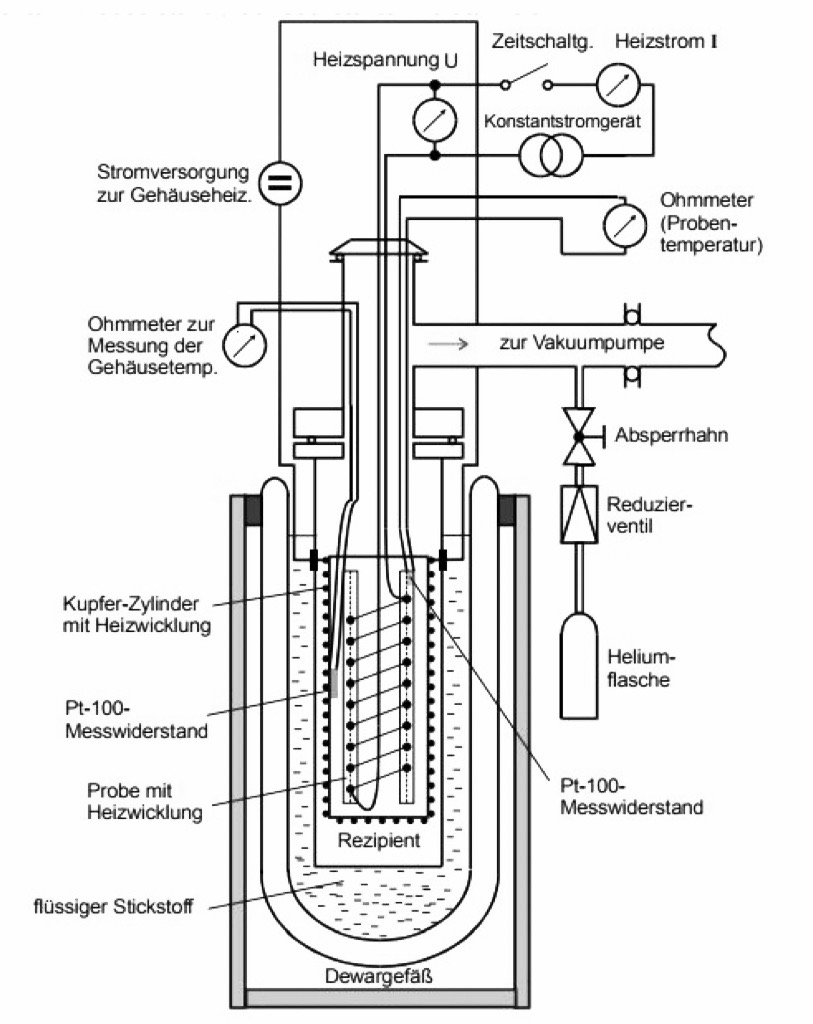
\includegraphics[width=0.46\linewidth]{content/graphics/equipment.jpg}
	\caption{Schematic depiction of the measuring apparatus. \cite{molar_heat}}
	\label{fig:equipment}
\end{figure}
